\documentclass{article}[14pt, letterpaper, Times New Roman]
\usepackage{graphicx}
\graphicspath{ {images/} }
\usepackage{listings}
\usepackage{geometry}
\geometry{margin=1in}

\title{2P04 Lab 4}
\author{Talha Ahmad, 400517273}

\begin{document}

\maketitle

\section{Lecture 12}

\subsection{Lecture Questions}

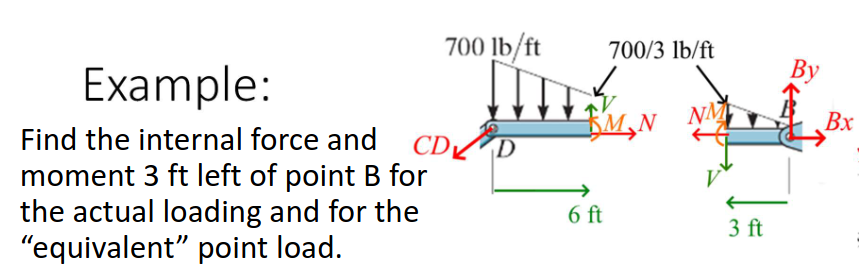
\includegraphics[width=15cm]{l12-lq.png}

We can start by first solving for this system as a whole without considering the internal forces.
Then, we can switch and use one half of the right side where we can consider the internal forces and in doing so, we can solve for the internal forces.
We can write out the following Maple code for this:

\begin{lstlisting}[language=matlab]
# Lecture 12 lecture question

# Solve for outside values
restart: p:=700*(1-x/9):
solve([
-CD*4/5+Bx,
-CD*3/5-int(p,x=0..9)+By,
-int(x*p,x=0..9)+9*By]); assign(%):

# Solve for internal values
solve([
-4/5*CD+N,
-3/5*CD-int(p,x=0..6)+V,
-int(x*p,x=0..6)+6*V+M]);
\end{lstlisting}

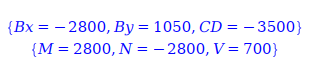
\includegraphics[width=8cm]{l12-lq-o.png}

Therefore, we get that the shear force at the internal point is 700 N upwards, the normal force is 2800 N towards the right, and the moment is 2800 N*m out of the page.

\subsection{Quiz and Reflection}

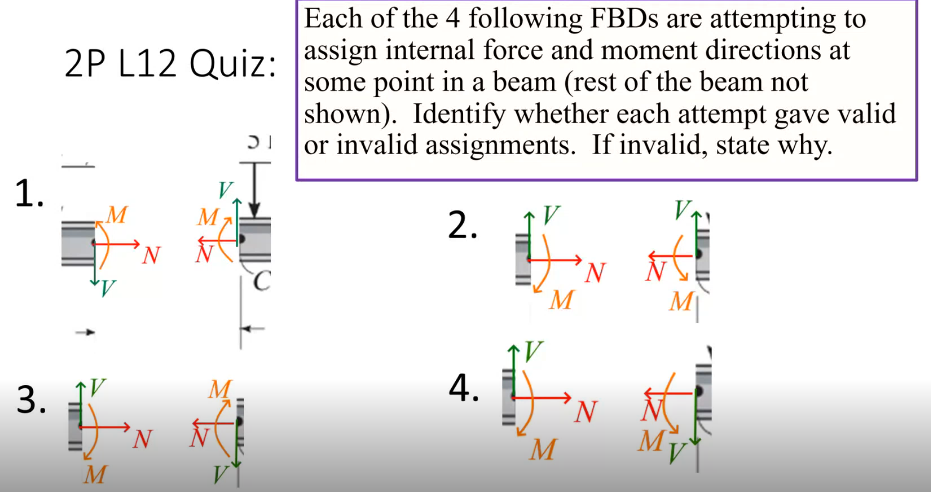
\includegraphics[width=15cm]{l12-quiz.png}

Assignment 1: Valid since Newton's third law is applied here.

\medskip

Assignment 2: Invalid since the sheer force at one point does not oppose the sheer force at another point.
Violates Newton's third law.

\medskip

Assignment 3: Invalid since the Moment's are both clockwise and do not oppose each other.

\medskip

Assignment 4: Valid since Newton's 3rd law is applied here.

\medskip

Reflection: In this lecture, we learned about how to solve for internal forces in a system by first solving for the system as a whole and then solving for the internal forces. This is a very useful technique that can be used to solve for internal forces in a system.

\subsection{Question Bank Problems}

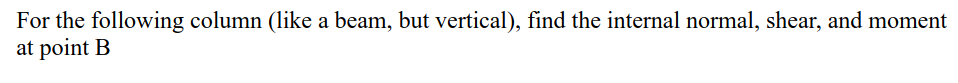
\includegraphics[width=15cm]{l12-pbq1.png}

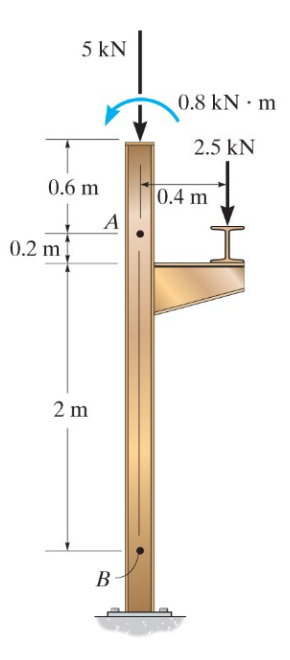
\includegraphics[width=8cm]{l12-pbq2.png}

When solving this problem in our Maple code, we can assume that, at point B, the normal is upwards, the sheer force is to the right, and the moment is into the page.
These points are arbitrary since if we assume the opposite, we will get the same answer but with the opposite sign.
With these facts, we can write out our Maple code as follows:

\begin{lstlisting}[language=matlab]
restart:
solve([
-2.5-5+N,
0.8-0.4*2.5-M,
V], [V,N,M]);
\end{lstlisting}


\includegraphics[width=15cm]{l12-pbq-o.png}

We can see that the sheer force is 0 N, the normal force is 7.5 N upwards, and the moment is 0.2 N*m out of the page.

\section{Lecture 13}

\subsection{Lecture Questions}

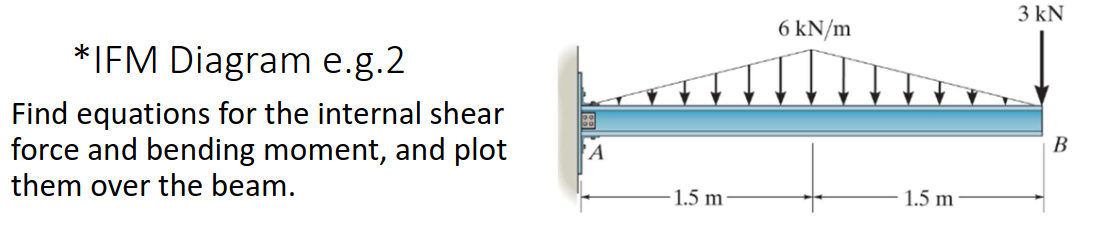
\includegraphics[width=15cm]{l13-lq.png}

We can move from left to right which means that we need to solve for the reaction forces at point A.
Given the reaction forces, we can then move left to right and solve for the moment and the sheer force.
The following Maple code can be used to solve this:

\begin{lstlisting}[language=matlab]
restart: p:=piecewise(x<1.5, 6*x/1.5, x>=1.5, 12-6*x/1.5):
solve([
Ay-int(p,x=0..3)-3,
MA-int(x*p,x=0..3)-3*3]): assign(%);
solve([
Ay-int(p,x=0..x)+V,
MA-int(x*p,x=0..x)+x*V+M], [V,M]): assign(%):
plot([V,M], x=0..3);
\end{lstlisting}

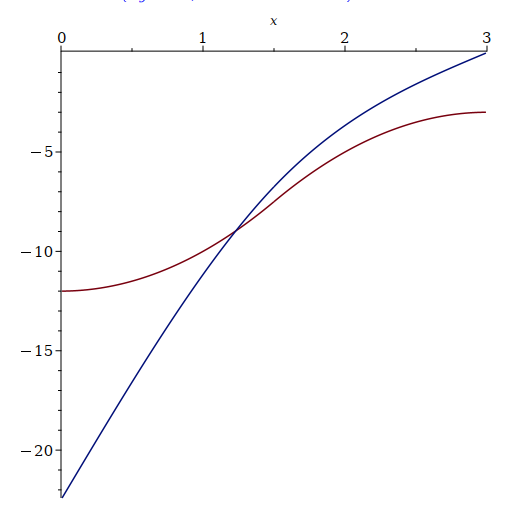
\includegraphics[width=15cm]{l13-lq-o.png}

We have a plot for the sheer force and the moment as a function of x.

\subsection{Quiz and Reflection}

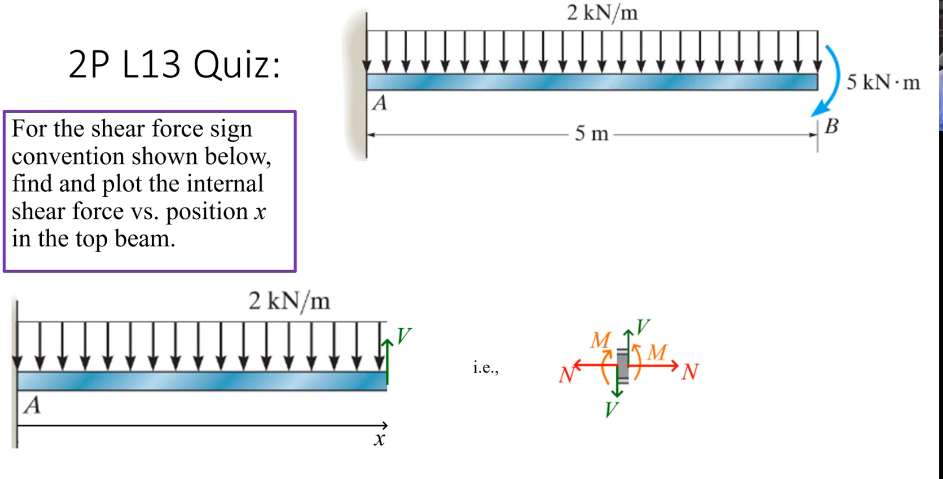
\includegraphics[width=15cm]{l13-quiz.png}

We can start by solving for the reaction forces at point A.
Then, we can move from left to right and solve for the moment and the sheer force.
The following Maple code can be used to solve this:

\begin{lstlisting}[language=matlab]
# Quiz
restart:
solve([Ay-int(2,x=0..5)], Ay); assign(%);

solve([Ay+V-int(2, x=0..x)], [V]);
assign(%); plot(V, x=0..5);
\end{lstlisting}

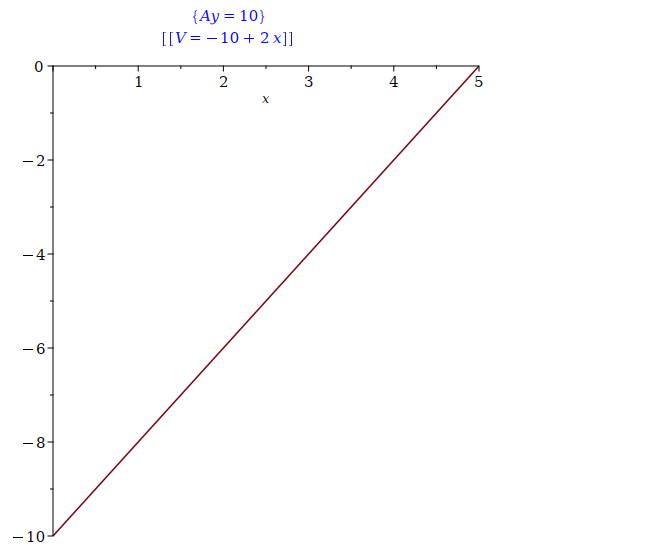
\includegraphics[width=15cm]{l13-quiz-o.png}

We can see that the sheer force goes to 0 as we travel from left to right.

\medskip

Reflection: In this lecture, we learned about how to solve for the reaction forces at a point and then move from left to right to solve for the moment and the sheer force. This is a very useful technique that can be used to solve for the moment and sheer force in a system.

\subsection{Question Bank Problems}

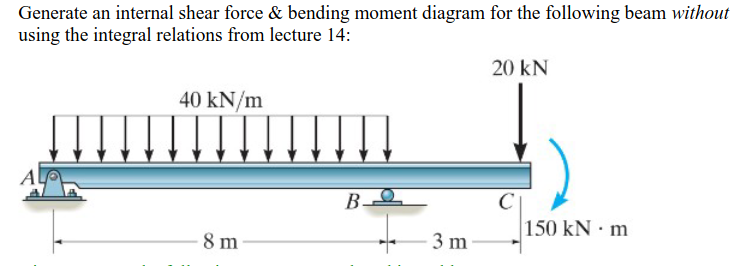
\includegraphics[width=15cm]{l13-pbq.png}

We can start by start by solving for the reactions at at points A and B.
Given those reactions, we can proceed and solve for the moment and the sheer force as we move from left to right.

For the reaction forces, at point B we have a single reaction force that is upwards.
At point A, we have a normal force upwards and a force to the right.
In the event that either force is negative, we can assume that the force is in the opposite direction.

In regards to directions for the sheer force and moment, we can assume that the sheer force is acting upwards and the moment is out	of the page.

For the By force in the context of the sheer force, we only need to consider at x=8.

We can now write out our Maple code to solve this:

\begin{lstlisting}[language=matlab]
# Lecture 13 Problem Bank Question
restart:
p:=piecewise(x<8,40):
solve([
Ay+By-int(p, x=0..11)-20,
Ax, # Only x force
-int(x*p,x=0..11)+8*By-11*20-150], [Ax,Ay,By]); assign(%);

# Now solve for sheer force

solve([
Ay-int(p,x=0..x)+piecewise(x=8, By)+V,
-int(x*p,x=0..x)+piecewise(x=8, By*8)+x*V+M], [M, V]); assign(%);
plot([V,M], x=0..11);
\end{lstlisting}

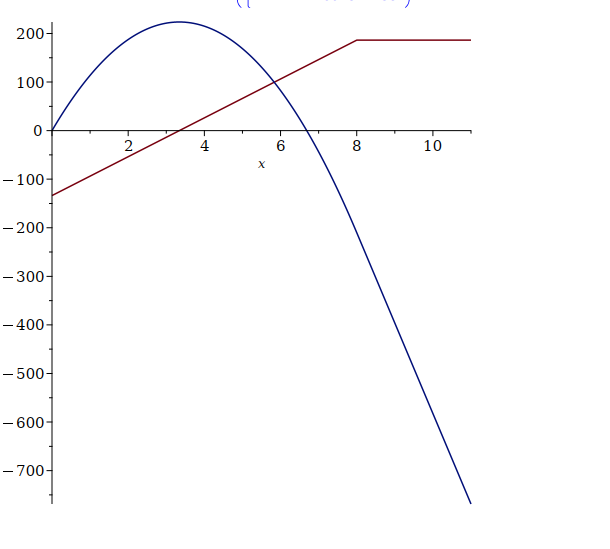
\includegraphics[width=15cm]{l13-pbq-o.png}

We can see that initially the sheer force (red) is pointing down, but it eventually becomes more positive before reaching an upper limit once no new forces are being introduced.

In regards to the moment, it initially starts at 0, then increases to a maximum point before continuously decreasing to a lower and lower value depending on the distance at which we calculate it.

The negative moment means that it's acting into the page since it was assumed that the moment was acting out of the page in our initial assumptions.


\end{document}

